%%%design overview over libpninx

The aim of \pninx\ is to provide an easy to use but yet powerful interface
to write Nexus files from C++. Although the Nexus group already provides 
an binding of their Nexus API (NAPI) for C++, this is not much more than a 
thin wrapper around the C library. Thus the native C++ API suffers from 
a whole bunch of features that a C++ programmer would expect from an API. 
\pninx\ is an approach to overcome the limitations of the native C++ API 
and provide you with all the object oriented features that C++ exposes.

In this chapter the general design of the library will be discussed. 
Though this section is usualy for developers only, users of the library 
are highly encouraged to read this chapter as it provides a lot of useful 
information about the philosophy behind certain objects. In particular 
section~\ref{section:nxfield_design} should be read by all users of \pninx. 

\section{Classes and implementation}\label{section:classes_implementation}

%%%----------------------------------------------------------------------------
\begin{figure}[tb]
\centering
\begin{minipage}[c]{0.5\linewidth}
\centering
\resizebox{\linewidth}{!}{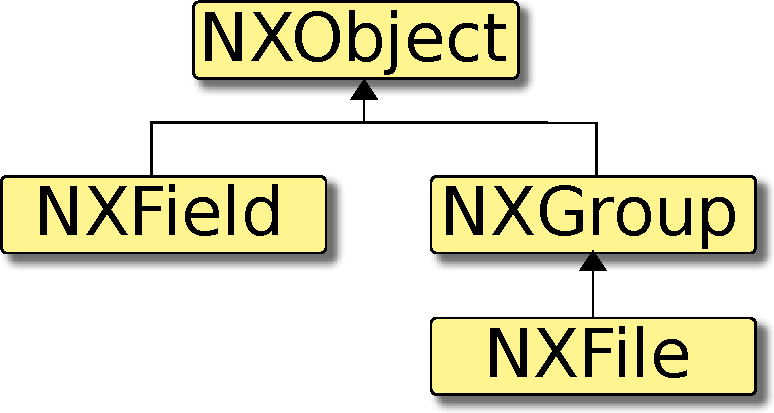
\includegraphics{pics/class_inheritance.pdf}}
\end{minipage}
\hfill
\begin{minipage}[c]{0.49\linewidth}
\caption{{\small\label{fig:class_inheritance}
Inheritance relations between the major objects provided by \pninx.
\nxobject\ is the root of the class tree but will hardly be used. 
The class important to a developer are the three classes derived from 
\nxobject: \nxfield, \nxgroup, and \nxfile.
}}
\end{minipage}
\end{figure}
%%%----------------------------------------------------------------------------
In order to remain simple to use \pninx\ exposes only four classes to the 
user where only three are needed in real world applications in order to 
read and write data. 
Figure~\ref{fig:class_inheritance} shows the inheritance tree of the 
exposed classes. The top-level object is \nxobject. This class 
collates all methods common to each object in the tree. However, you hardly 
ever use \nxobject\ in your code. The only classes relevant for users
are
\begin{description}
\item[\nxgroup] the standard container to hold all kinds of objects
\item[\nxfield] the data holding objects
\item[\nxfile] object representing a data file.
\end{description}
\nxfile is a descandent of \nxgroup\ as can be seen in
Fig.~\ref{fig:class_inheritance}. Thus it posses all the functionality that 
\nxgroup\ has aside from those methods necessary for file handling. 
\pninx\ uses HDF5 to write data to disk. However, you do not have to know 
anything about HDF5. No low level HDF5 calls are necessary. Everything is 
masked by the three objects mentioned above. 
In order to do so a Bridge pattern~\cite{book:gof} was used for the
implementation. The idea was to separate the interface provided to the user from the 
concrete interface used to communicate with the HDF5 library. 
This allows us to change the HDF5 backend completely without changing 
user code using the library (maybe recompilation is needed - but this is not as
bad as changing code). This gives us much more freedom in maintaining \pninx.
The bridge pattern is not implemented as shown in \cite{book:gof} but rather 
by using a template approach as shown  in \cite{book:alexandrescu}.
Hence the code remains free of pointers which makes it much more readable. 
Furthermore it should be mentioned that the \pninx\ heavily relies on features 
provided by the C++11 standard. Thus, an actuall compiler is required to 
build the library.
 

\section{A closer view on \nxfield}\label{section:nxfield_design}
\nxfield\ is most probably the most important object in the \pninx-universe. 
Objects of type \nxfield\ are used to read from and write data to the file. 
From the point of C++, \nxfield\ can be considered a container like 
{\tt std::vector<>} or {\tt std::list<>}.
When an \nxfield\ object is newly instantiated it represents an empty container. 
Writing data to disk means nothing else than appending data to the container. 
To read data form disk means to fetch data from the container.
The size (number of elements) of the container is limited by the amount of 
free space on the storage device on which the file is writen.
\nxfield\ mimics up to some point the behavior of the container objects
provided by the C++ standard library. So you will find methods like 
{\tt get()}, {\tt set()}, {\tt append()} and so on. 
There are basically three kinds of objects that can be stored in this container
\begin{enumerate}
  \item numerical data
  \item strings
  \item and binary uninterpreted data.
\end{enumerate}
\nxfield\ can handle all different kinds of data which keeps the number of 
classes in the library small. However, there is a price one has to pay 
for this simplicity: \nxfield\ behaves slightly different depending 
on which kind of data is stored. 

\subsection{Numerical data}
%%%-----------------------------------------------------------------------------
\begin{figure}[tb]
\centering
\begin{minipage}[t]{0.39\linewidth}
\centering
\resizebox{\linewidth}{!}{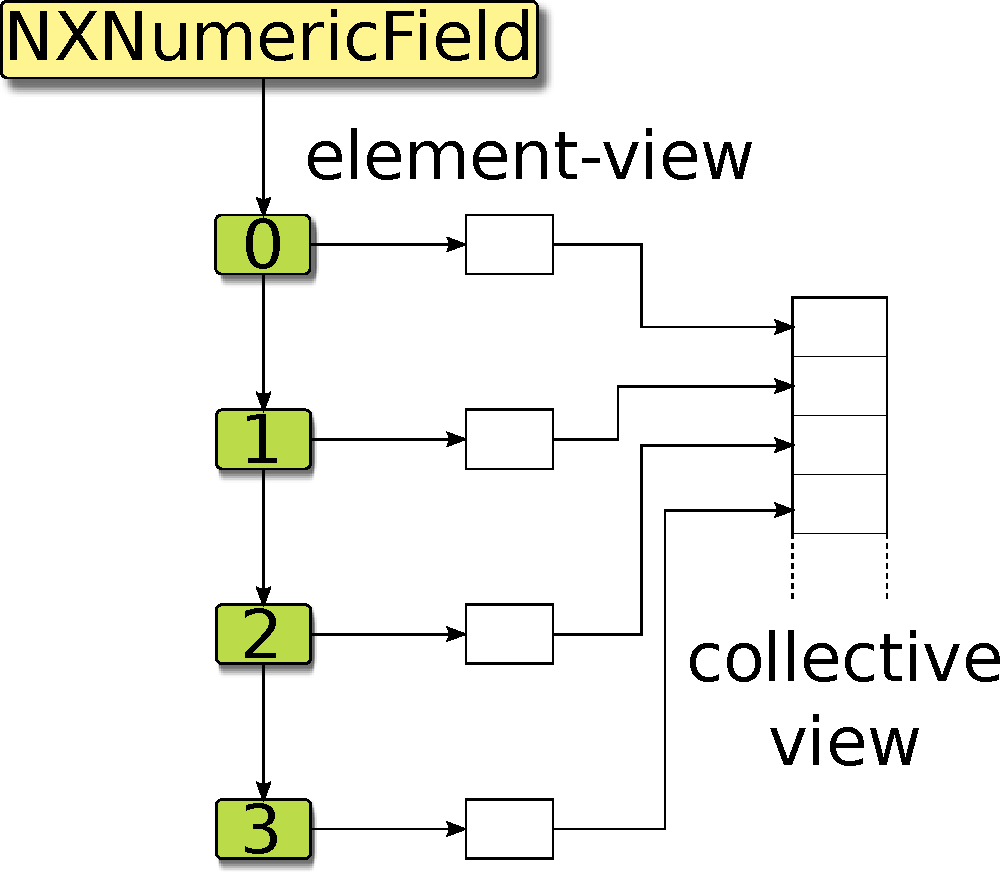
\includegraphics{pics/container_scalar.pdf}}
\caption{{\small\label{fig:container_scalar} An \nxfield\ object holding 
scalar values can be either considered as a list of single scalar values 
or as a 1-dimensional array of numbers.}}
\end{minipage}
\hfill
\begin{minipage}[t]{0.58\linewidth}
\centering
\resizebox{\linewidth}{!}{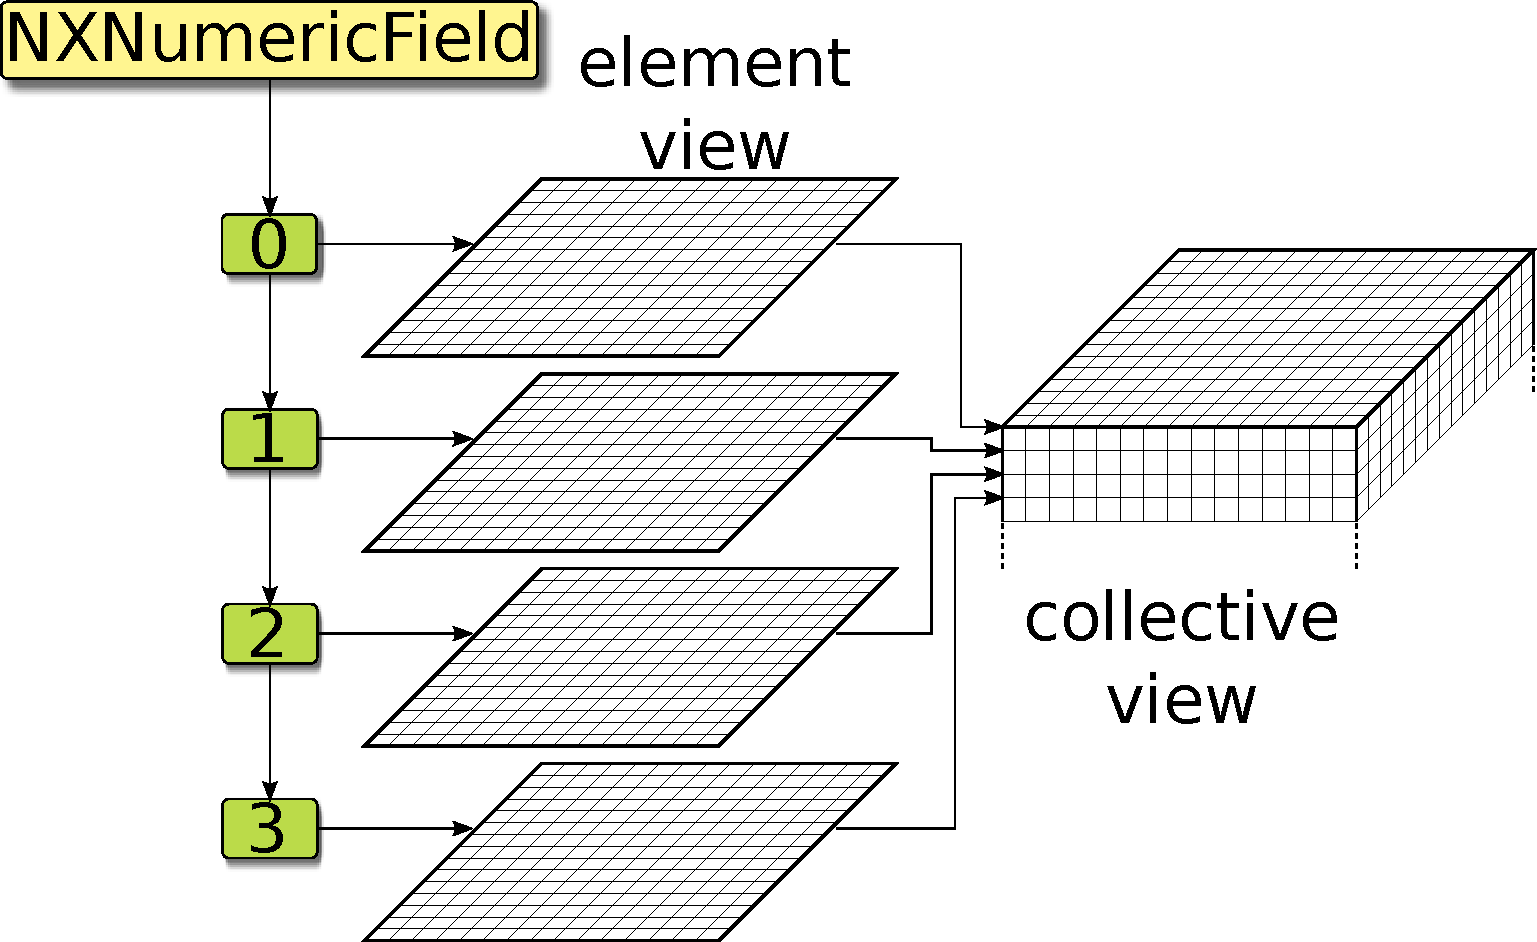
\includegraphics{pics/container_array.pdf}}
\caption{{\small\label{fig:container_array}An \nxfield\ object with 2D-arrays 
of data can be either considered as a list of individual arrays or as a
single 3D array where the first dimension runs over the number of elements
and the other dimension correspond to those of the array data.}}
\end{minipage}
\end{figure} 
%%%-----------------------------------------------------------------------------
Numeric data is handled by the two templates \arrayt\ and \scalart\  
provided by \pniutils. For more information on this two templates see 
the users-guide of \pniutils.
Figures~\ref{fig:container_scalar} and \ref{fig:container_array} show how these 
two templates are stored in a field container. 
Basically we can treat data in two different ways: as a list of invididual
elements or, collectively, as a single array of data. 
Both approaches are are depicted in Figs.~\ref{fig:container_scalar} and 
\ref{fig:container_array}. A field storing scalars can be either considered 
as a list of individual numbers or as a 1D array of numbers. 
The same holds for arrays as shown in Fig.~\ref{fig:container_array}. Here 
we have either a list of individual 2D arrays or a single 3D array where the 
first index runs over the number of elements in the list while the remaining 
indices correspond to those of the 2D arrays.
Both points of view - the element wise or the collective view have their own 
applications and thus are taken into account in the API. 

\subsection{String data}
%%%-----------------------------------------------------------------------------
\begin{figure}[tb]
\centering
\begin{minipage}[c]{0.4\linewidth}
\centering
\resizebox{\linewidth}{!}{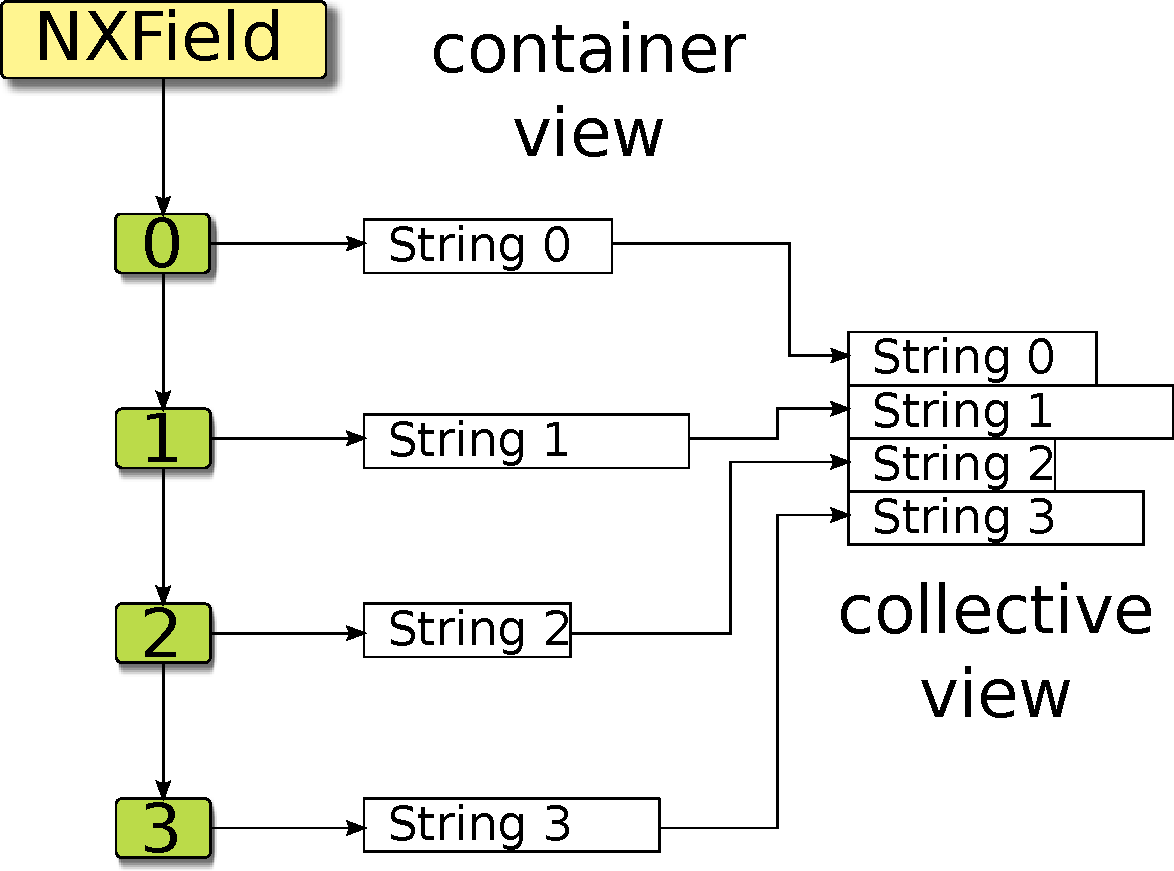
\includegraphics{pics/container_string.pdf}}
\end{minipage}
\hfill
\begin{minipage}[c]{0.58\linewidth}
\caption{{\small\label{fig:container_string} String fields can hold strings 
of different length. Each time a string is appended to the container 
a new entry is created. This can be used to store text files in a line-wise
manner. Each entry represents a line in the text-file.}}
\end{minipage}
\end{figure}
%%%-----------------------------------------------------------------------------
As usually strings are slightly different from everything else. 
This is also true for \pninx\ as shwon in Fig.~\ref{fig:container_string}.
In the container view each element stores an individual string. The strings 
can have different length. 
As for numeric data one can either read individual strings or all strings 
in a single step. This would make it easy for instance to dump an entire 
ASCII file in such a string field. 

\subsection{Binary data}
%%%-----------------------------------------------------------------------------
\begin{figure}[tb]
\centering
\begin{minipage}[c]{0.4\linewidth}
\centering
\resizebox{\linewidth}{!}{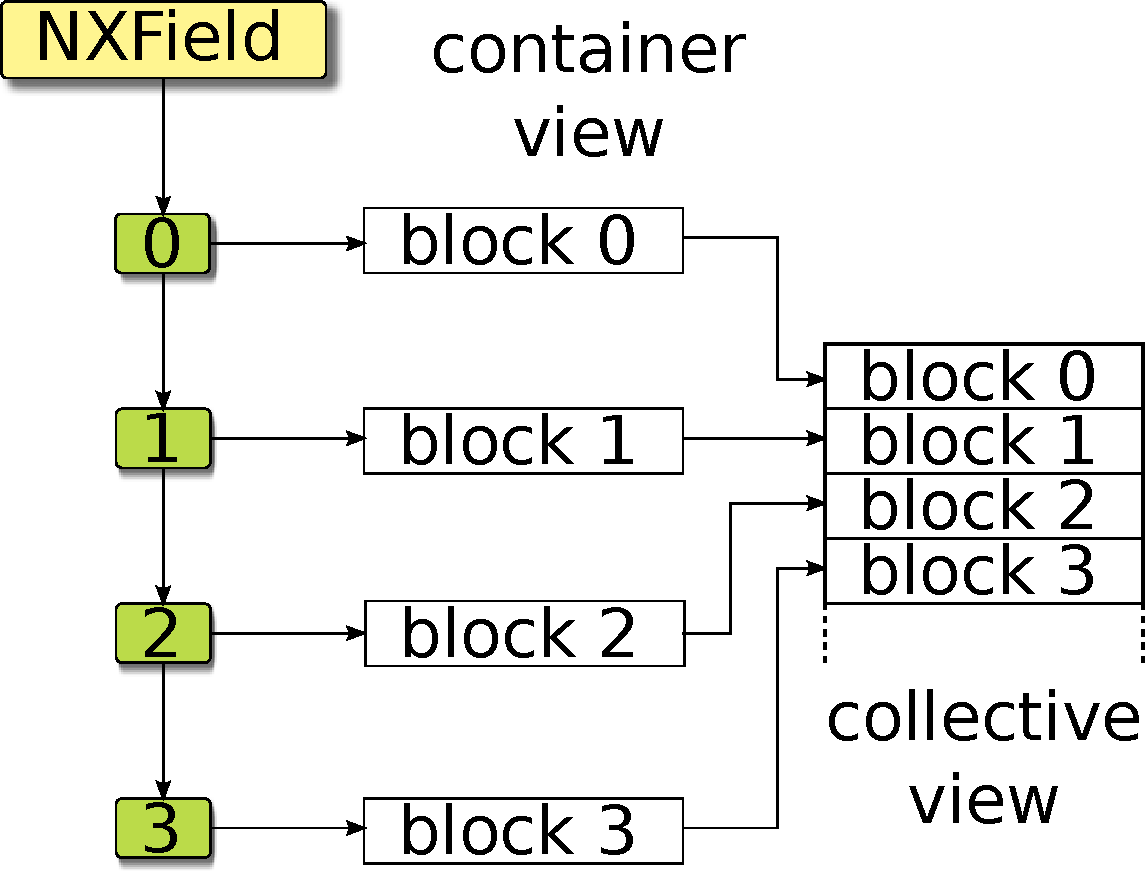
\includegraphics{pics/container_binary.pdf}}
\end{minipage}
\hfill
\begin{minipage}[c]{0.58\linewidth}
\caption{{\small\label{fig:container_binary} Binary data is stored block wise.
Each container entry holds a block of constant size of data. Thus at 
field creation a block size must be passed to the creating factory method. 
If the block size is as large as the entire binary data only a single element 
must be stored representing the entire binary data.}}
\end{minipage}
\end{figure}
%%%-----------------------------------------------------------------------------
The last class of data supported by Nexus is binary data. 
Image files (JPEG, PNG,TIFF), PDF files or other binary data can be stored in
such a field. The binary stream is not interpreted. 
The interesting question is how to represent such a binary blob of data in 
a container view as it is provided by \nxfield?. 
Binary data is usually read in blocks of a certain size. So the elements
in the list are blocks. In the simplest case a block is only $1$ byte. 
In this case you can read data byte by byte and dump it to the field. 




 

